	
	\documentclass[12pt,journal,compsoc]{IEEEtran}
	\usepackage[utf8]{inputenc}

	% *** CITATION PACKAGES ***
	\usepackage[nocompress]{cite}
	%\usepackage{cite}

	% *** GRAPHICS RELATED PACKAGES ***
	\usepackage[pdftex]{graphicx}
	\graphicspath{{img/}}
	\DeclareGraphicsExtensions{.pdf,.jpeg,.jpg,.png}

	% *** MATH PACKAGES ***
	\usepackage[cmex10]{amsmath}

	% *** SPECIALIZED LIST PACKAGES ***
	\usepackage[footnote]{acronym}
	\usepackage{algorithmic}

	% *** ALIGNMENT PACKAGES ***
	\usepackage{array}
	\usepackage{mdwmath}
	\usepackage{mdwtab}
	\usepackage{eqparbox}

	% *** SUBFIGURE PACKAGES ***
	\usepackage[caption=false,font=normalsize,labelfont=sf,textfont=sf]{subfig}
	%\usepackage[caption=false,font=footnotesize]{subfig}

	% *** FLOAT PACKAGES ***
	\usepackage{dblfloatfix}

	% *** PDF, URL AND HYPERLINK PACKAGES ***
	\usepackage{url}

	\newcommand\MYhyperrefoptions{bookmarks=true,bookmarksnumbered=true,
	pdfpagemode={UseOutlines},plainpages=false,pdfpagelabels=true,
	colorlinks=true,linkcolor={black},citecolor={black},urlcolor={black},
	pdftitle={Efficient 3D Isotropic Volume Reconstruction Based On 2D Localized Ultrasound Images},
	pdfsubject={Introduction To Lab Research},
	pdfauthor={Keck Jean-Baptiste},
pdfkeywords={TIMC-IMAG, Introduction to Lab Research, Arthrosis, Ensimag, CUDA, GPGPU, Ultrasound Imaging, Isotropic Volume Reconstruction, Report}}
	

        \acrodef{gpgpu}[GPGPU]{General Purpose Computing on Graphics Processing Unit}
        \acrodef{cuda}[CUDA]{Compute Unified Device Architecture}
        \acrodef{timcimag}[TIMC-IMAG]{Techniques de l’Ingénierie Médicale et de la Complexité - Informatique, Mathématiques et Applications, Grenoble}
        \acrodef{gmcao}[GMCAO]{Gestes Médico-Chirurgicaux Assistés par Ordinateur}

	\begin{document}

	\title{Efficient 3D Isotropic Volume Reconstruction Based On 2D Localized Ultrasound Images}

	\author{Jean-Baptiste Keck,~\IEEEmembership{Student,~Ensimag}\\
		Matthieu Chabanas,~\IEEEmembership{Supervisor,~TIMC-IMAG Laboratory}

	\IEEEcompsocitemizethanks{
	\IEEEcompsocthanksitem M. ~Keck is a student at Ensimag, Grenoble, France.
	\IEEEcompsocthanksitem M. ~Chabanas is in the team Gestes Médico-Chirurgicaux Assistés par Ordinateur in the TIMC-IMAG Laboratory, University of Grenoble, France. He was my supervisor for this project.}
	}


	% The paper headers
	\markboth{Introduction to Laboratory Research, Report,~Version.~1, No.~1, May~2014}
	{Shell \MakeLowercase{\textit{et al.}}: Bare Advanced Demo of IEEEtran.cls for Journals}
	%\IEEEspecialpapernotice{IRL Report}

\IEEEtitleabstractindextext{%
\begin{abstract}
	A miniature 3D tracked ultrasonic probe has been developped to aquire intra-articular cartilage images under artroscopic chirurgy conditions. The aim is to detect cartilaginous lesions (arthrosis) and quantize their precise sizes and locations to help the clinician in his diagnostic and his therapeutic decision making.
	The ultrasonic transducer is tracked by an optical sensor, wich permits to find location and orientation of each 2D US images in a common 3D spacial reference. Near two thousands images are acquired when scanning a cartilage surface. An interesting tool is to rebuild a 3D isotropic volume (cubic voxels) with those images, allowing further processing.
	Conventional 3D ultrasound algorithms have low computational complexity but the huge amount of data generated makes it difficult to compute results within reasonable time on classical computers. In this paper we investigate the possibilities of regenerating a 3D isotropic volume with the help of \ac{gpgpu} (\ac{cuda}) by adaptating existing algorithms to massive parallelism provided by modern everyday GPUs.
\end{abstract}

% Note that keywords are not normally used for peerreview papers.
\begin{IEEEkeywords}
	TIMC-IMAG, Introduction to Lab Research, Arthrosis, Ensimag, \acl{cuda}, \acl{gpgpu}, Ultrasound Imaging, Isotropic Volume Reconstruction, Report.
\end{IEEEkeywords}}


% make the title area
\maketitle

\section{Introduction}

\IEEEPARstart{F}{reehand} three-dimentional ultrasound imaging is a highly attractive research area because it is capable of volumetric visualization and analysis of tissue and organs. Conventional two-dimentional ultrasound imaging has been widely used for many clinical applications such as medical diagnosis and image-guided surgery. In comparisson with Computed Tomography (CT) and Magnetic Resonance Imaging (MRI), ultrasound imaging is non invasive, real time, portable and low cost. However, 2D ultrasound imaging fails to offer clinicians whole volume data for visualization and analysis. Thus three-dimensional ultrasound imaging systems has been developped to overcome those limitations by constructing various 3D datasets. Several approaches for constructing 3D ultrasound volume data have been reported. These approaches can be classified into three categories : dedicated 3D probes, mechanical scanning approach, and freehand scaning approach. 
Dedicated 3D probes can provide 3D data in real time but they are expensive and have limitations in scanning large volume organs.
The mechanical scanning approaches usually use conventionals 2D transducers wich are translated and rotated with stepping motors. This design creates limitations in term of their scanning range. 
Finally, freehand ultrasound use conventionals 2D tranducers in pair with a positioning sensor to save position and orientation of each acquired image.
Freehand 3D ultrasound has received increasing attention for it's low-cost and flexibility, as it allows the user to manipulate and view the desired anatomical section freely.
During scanning a sequence of US images are captured along with their positions and orientations, asynchronously. Those datas are then used to reconstruct a 3D volume by using various interpolation or approximation algorithms. The reconstruction algorithm plays a key role in the construction of three-dimentional ultrasound volume data with higher image quality and faster reconstruction speed.\\

TODO\\

Even if conventional 3D reconstruction algorithms have low computational complexity, the huge amount of data generated by a single scan (thousands of 2D images) makes it difficult to compute volume data in reasonable clinical time on classical computers.
This paper aims to speed up 3D volume processing by adapting existing reconstruction algorithms to the massive parallelism provided by nowadays affordable GPUs. This is achieved throught \acl{gpgpu} (\ac{gpgpu}), a concept that has been well developped and widely adopted during the last decade and that continues its growth.
The Open Computing Language (OpenCL) is the currently dominant open general-purpose GPU computing language. The dominant proprietary framework is the \acl{cuda} (\ac{cuda}).
Althought \ac{cuda} requires a Nvidia CUDA compatible graphic card, we choose it because of its more mature status (performance and debugging tools) but algorithms are easily adaptable to OpenCL as well.

\section{System overview}

\subsection{System setup}

The freehand 3D ultrasound imaging system consits of three modules : a 2D ultrasound scanner specially designed to acquire intra-articular cartilage US images under artroscopic chirurgy conditions, an optical position and orientation sensor and a work station with custom-designed software for data-aquisition. The volume reconstruction is for the moment done as a post-process in another specially-designed piece of software.
The portable ultrasound scanner concists of 64 axis-aligned transducers. Althought it is a freehand system, the axe is slightly rotated by a stepper motor to achieve a greater scanning area. The transformation due to the rotation of the motor is taken in account.

\begin{figure}[!h]
\centering
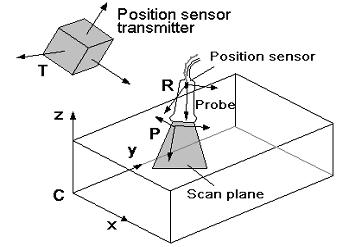
\includegraphics[width=2.5in]{freehand}
\caption{A classical freehand ultrasound imaging system setup}
\label{fig_1}
\end{figure}

The receiver of the spacial sensing device is attached to the hand-help probe of the ultrasound scanner.
During data acquisition, spacial data and digitalized 2D scans are simulteanously recorded and collected.
Since the ultrasound probe and the spacial sensor are independent, the temporal delay between two data streams can not be avoided.

\subsection{Data acquisition}

After signal processing 2D slices of 64x1296 pixels are generated. As the transducers are $\epsilon_x=205\mu m$ wide, the images have a width of $64\;\epsilon_x=19.12mm$. The precision on the other axe is $\epsilon_y=18\mu m$ 

\begin{figure}[!h]
\centering
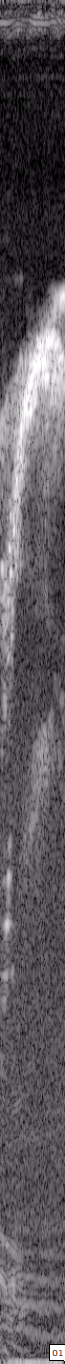
\includegraphics[width=40mm, height=50mm]{scan}
\caption{Typical 2D ultrasound image of intra articular cartilage. Image size : 64x1296 pixels, real size : 19.12x23.41mm}
\label{fig_2}
\end{figure}


\section{Reconstruction algorithms}



%\begin{figure*}[!t]
%\centering
%\subfloat[Case I]{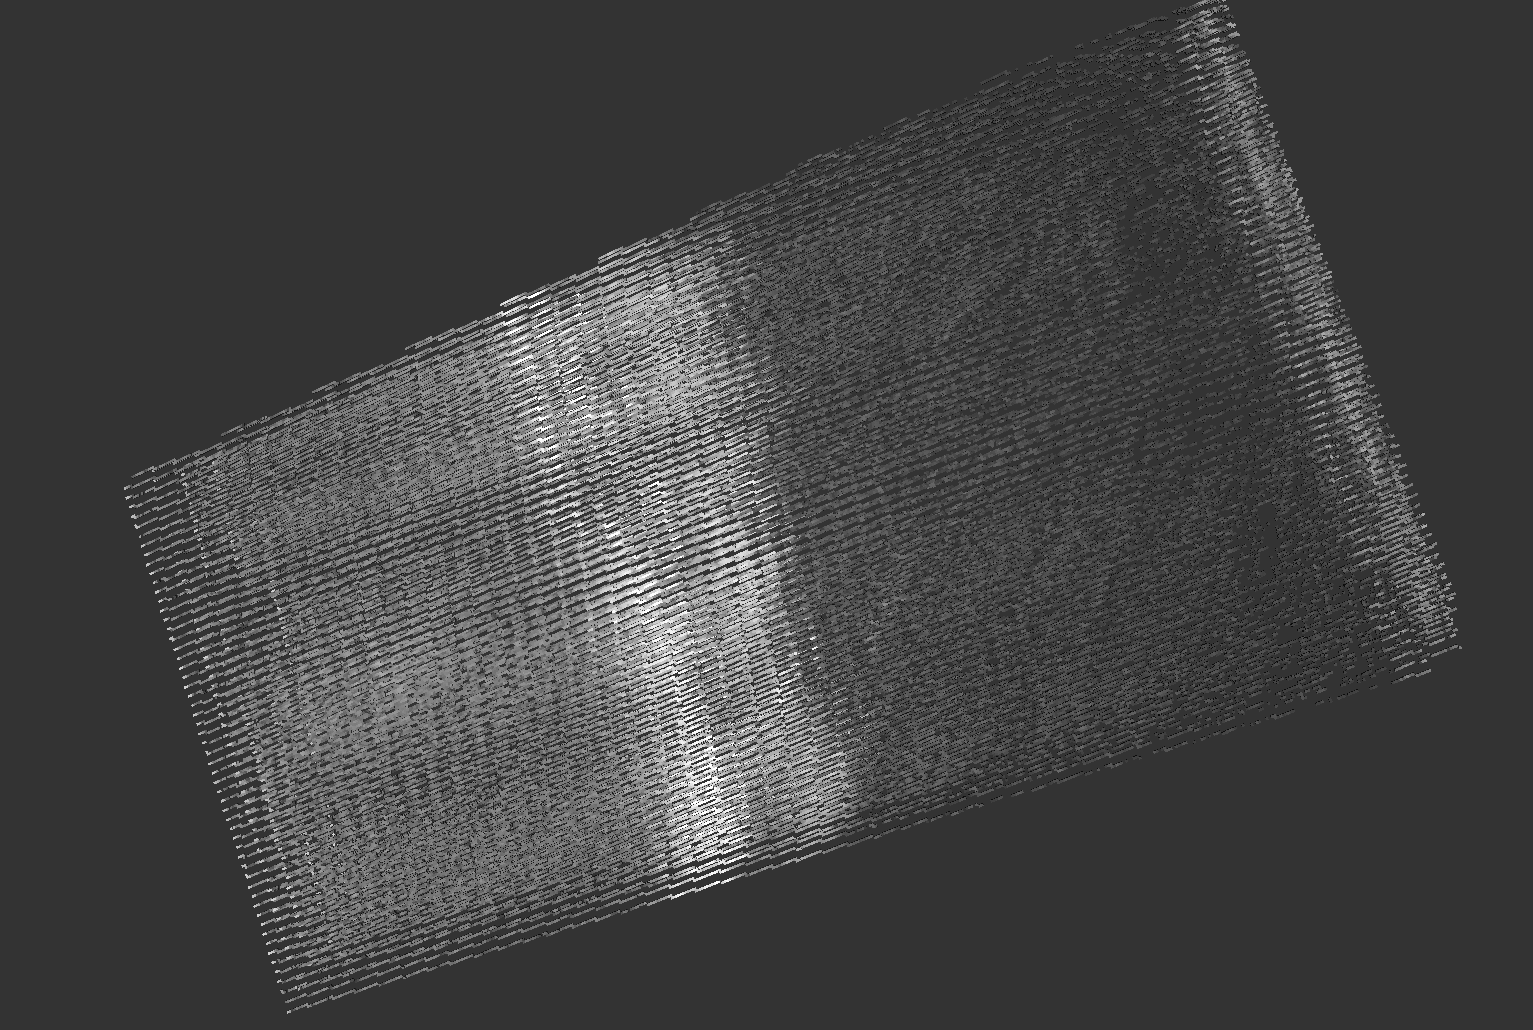
\includegraphics[width=1.5in]{data_0}%
%\label{fig_first_case}}
%\hfil
%\subfloat[Case II]{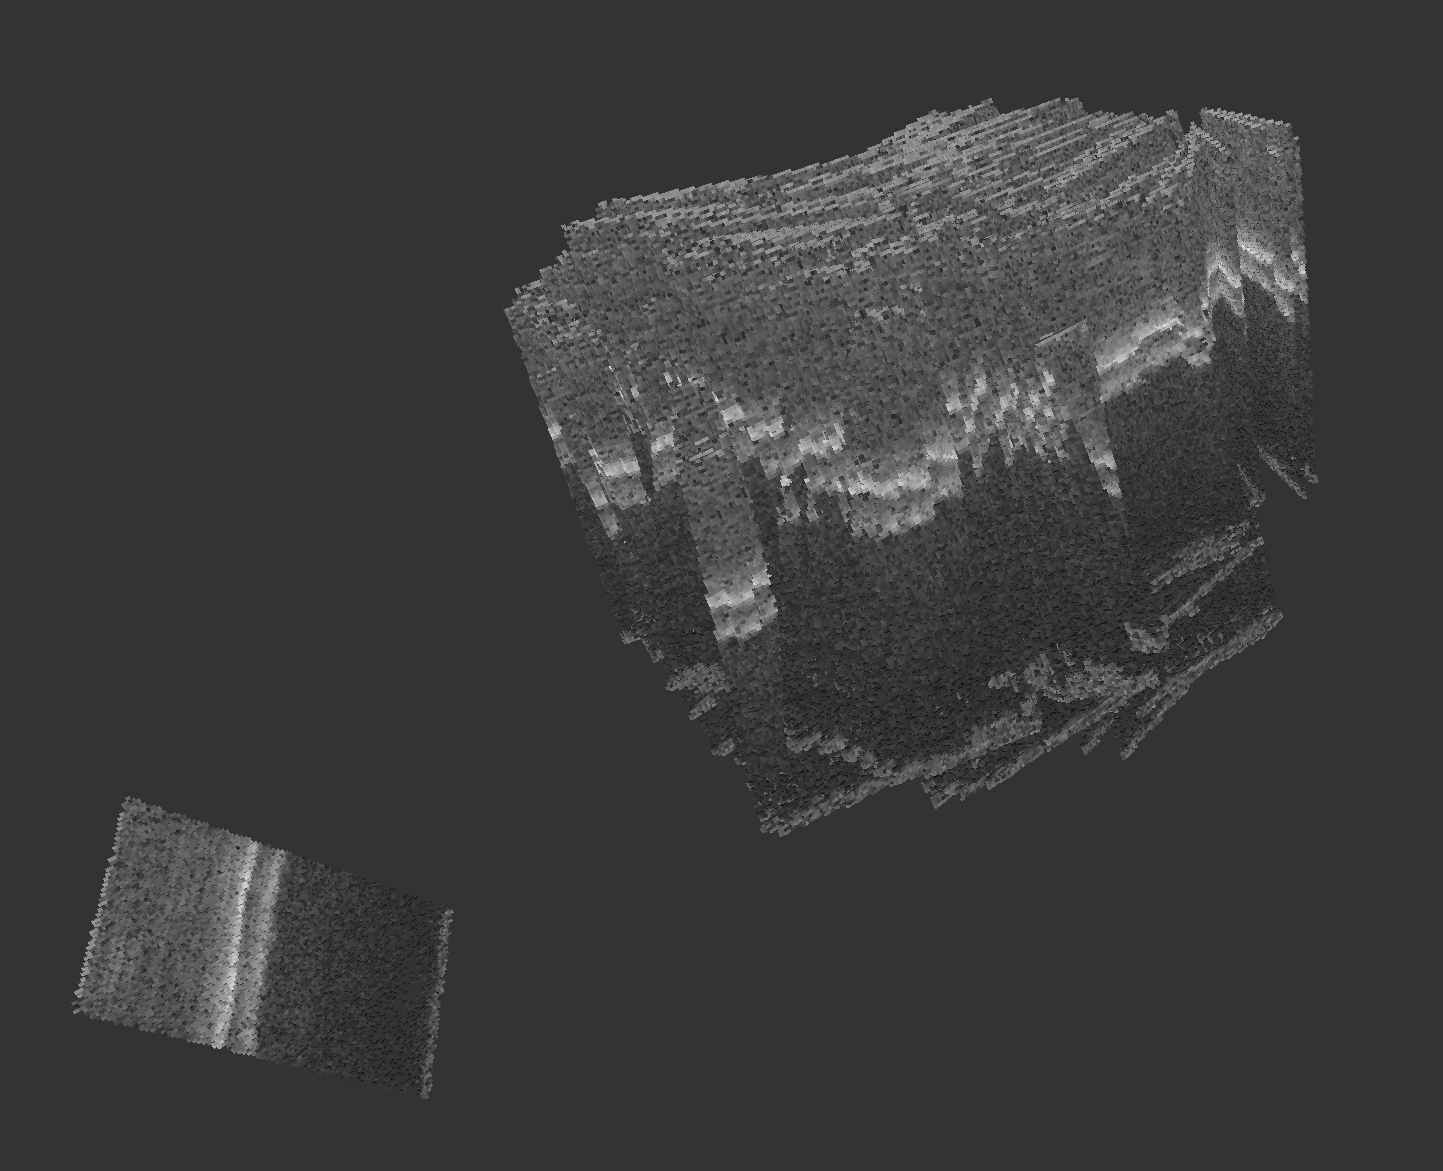
\includegraphics[width=1.5in]{data_1}%
%\label{fig_second_case}}
%\hfil
%\subfloat[Case III]{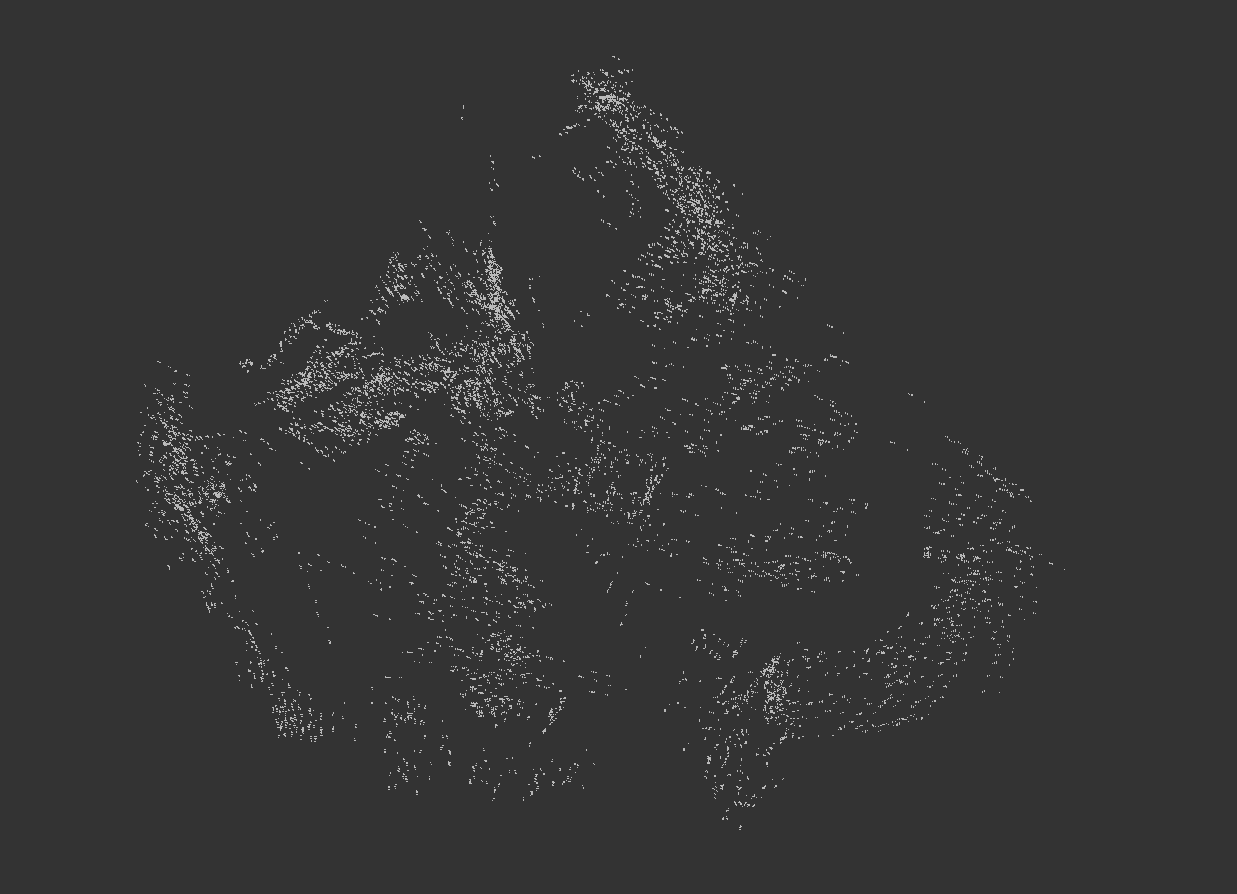
\includegraphics[width=1.5in]{femur_2}%
%\label{fig_third_case}}
%\caption{Simulation results.}
%\label{fig_sim2}
%\end{figure*}

%\begin{table}[!t]
%increase table row spacing, adjust to taste
%\renewcommand{\arraystretch}{1.3}
%if using array.sty, it might be a good idea to tweak the value of
%\extrarowheight as needed to properly center the text within the cells
%\caption{An Example of a Table}
%\label{table_example}
%\centering
%Some packages, such as MDW tools, offer better commands for making tables
%than the plain LaTeX2e tabular which is used here.
%\begin{tabular}{|c||c|}
%\hline
%One & Two\\
%\hline
%Three & Four\\
%\hline
%\end{tabular}
%\end{table}


\section{Conclusion}
The conclusion goes here.

\appendices
\section{Images Coordinate System}
appendix text goes here.

\section{Existing Hole Filling Algorithms}
appendix text goes here.

% you can choose not to have a title for an appendix
% if you want by leaving the argument blank
\section{Voxel Renderer}
Appendix text goes here.

\section*{Acknowledgments}
I would like to thank the TIMC-IMAG laboratory for having hosted me for 4 months, especially the GMCAO team members that were always here to help when there were any problems and for the good mood. Special thanks goes to M. Chabanas for having taken the time and energy throughout the project by providing precious feedbacks and for having introduced me to the TIMC-IMAG laboratory.

\cite{1}\cite{2}\cite{3}\cite{4}\cite{5}\cite{6}\cite{7}.

\bibliographystyle{IEEEtran}
\bibliography{master}


%\begin{IEEEbiography}[{\includegraphics[width=1in,height=1.25in,clip,keepaspectratio]{mshell}}]{Michael Shell}
%\begin{IEEEbiography}{Michael Shell}
%Biography text here.
%\end{IEEEbiography}

%\begin{IEEEbiographynophoto}{Jane Doe}
%Biography text here.
%\end{IEEEbiographynophoto}
%\vfill

\end{document}
